\section{Appendix}

%\subsection{}
%label{s:appendix:preemption}

%A few prior approaches~\cite{ski, snowboard, razzer} suspend a vCPU
%instead of a guest thread. While suspending a vCPU grants the ability
%to control an interleaving, it is not suitable for our purpose because
%suspending a vCPU may unexpectedly suspend another vCPU. An example we
%observed is TLB shootdown~\cite{tlbshootdown}. When a vCPU wants TLB
%shootdown, it sends inter-process interrupts (IPIs) to all cores and
%wait until all cores to execute the TLB shootdown handler.  In this
%case, if one vCPU is entirely suspended, the TLB shootdown cannot be
%successfully conducted causing the vCPU invoking TLB shootdown
%blocked.
%
%Therefore, instead of adopting the prior approach, our hypervisor is
%designed to suspends and resumes a guest thread.


\subsection{Hashing segment graph}
\label{s:appendix:hash}
% \dr{I want to discuss about this part. I'm thinking taking this part
%   out to the appendix section:}
% %
In particular, for all vertices $v$ in $V_i$, we first calculate a
hash value of $v$, $hash(v)$, which reflects its out-going edges. With
$o_1, ..., o_m$ that $v \rightarrow o_x \in E_i$,
%
%
\\[1pt]
\[
  hash(v) = \mathcal{H}(v.label {++} o_1.label {++} ... {++}
  o_m.label)
\]
\\[1pt]
%
where $\mathcal{H}$ denotes the
non-cryptographic FNV hash function~\cite{fnv, fnv-go}, and ${++}$
denotes the label-concatenation operation.
%
Then,
%
\\[1pt]
\[
  hash(g_i) = \underset{v \in V_i}{\oplus} hash(v)
\]
\\[1pt]
%
where $\oplus$ denotes the XOR operation.



\subsection{Input Transformation}
\label{s:appendix:inputtransform}



\subsection{Virtual Machine Introspection}
\label{s:appendix:vmi}


As a hardware breakpoint does not distinguish the running context of a
kernel, if the context switch happens, a breakpoint may be hit by
another thread or an interrupt handler, making the execution out of
expectation.
%
The hypervisor recognizes a running context using \texttt{task_struct}
which holds the thread description, and the per-cpu
\texttt{preempt_count} variable indicating what context the thread is
in (\eg, a task context for running a syscall, or a hardIRQ context to
handle hardware interrupts).
%
If a breakpoint is hit by a context other than the fuzzer-controlled
thread, our hypervisor ignores it and keeps the breakpoint.



When the suspended thread already acquires a lock while the running
thread wants to hold the same lock, the whole execution cannot make a
progress, because our hypervisor forces the lock-holding thread to
suspend.
%
Therefore, our hypervisor inspects whether the running thread is going
to be blocked due to the lock contention, and if it is, our hypervisor
takes control from the running thread to the suspended thread.
%
Inspecting the lock contention is conducted by hooking lockdep
functions~\cite{lockdep} that are commonly called from synchronization
prmitives.
%
When the lockdep functions are called, our hypervisor determins
whether the running thread can make a progress through various
information such as the address of the synchronization primitive, and
operation type (\ie, lock, unlock, and trylock).

\subsection{Data race and race conditions}
\label{s:appendix:datarace}


A concurrency bug can be classified into two categories according to
how it adversely affects a program.

\begin{figure}
  \centering
  \subfloat[Data race.\label{subfig:datarace}] {
    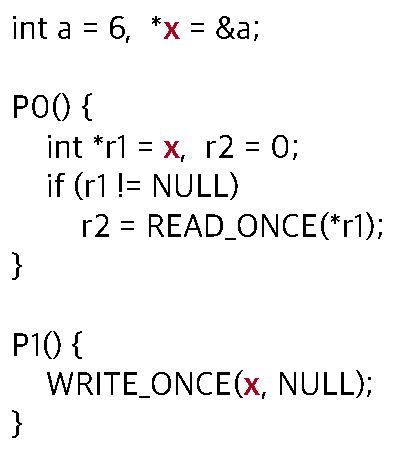
\includegraphics[width=0.45\linewidth]{fig/datarace.pdf}
  }
  \hfill
  \subfloat[Race condition.\label{subfig:racecondition}] {
    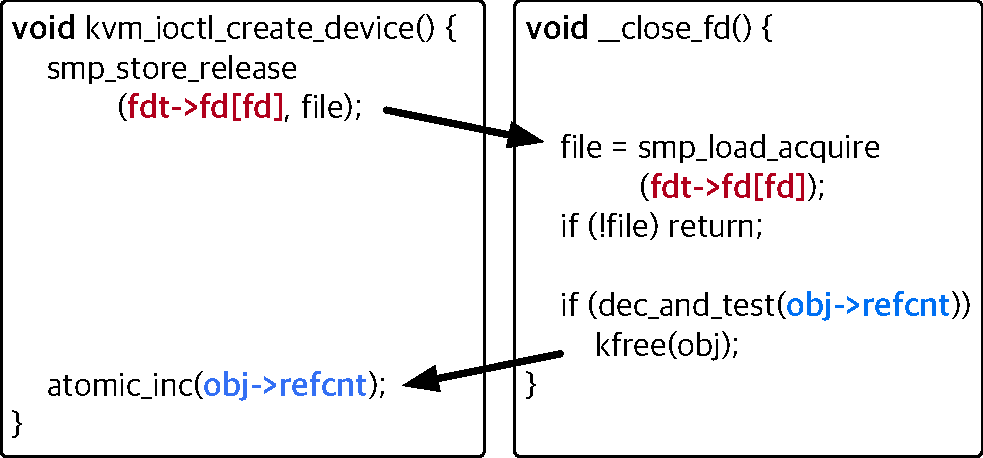
\includegraphics[width=0.45\linewidth]{fig/racecondition.pdf}
  }
  \caption{Two types of concurrency bugs.}
  \label{fig:concurrencybugs}
\end{figure}


\PP{Data race.}
%
Although the concept of data race is well known, its formal definition
depends on a programming language~\cite{C-standard-n2310,
  java-standard} or a program in development~\cite{lkmm}. In this
paper, we employ the definition from Linux Kernel Memory Model
(LKMM)~\cite{lkmm}. According to LKMM, a data race occurs when there
are two memory accesses such that 1) they access the same location, 2)
at least one of them is a store, 3) at least one of them is not
annotated with special operations such as \texttt{WRITE_ONCE()}, or
\texttt{smp_load_acquire()}, 4) they occur on different CPUs (or in
different threads on the same CPU), and 5) they execute concurrently.
%
Informally, a data race indicates un-annotated concurrent accesses to
a shared memory location.

Data races are problematic because they may confuse a compiler.  LKMM
allows a compiler to assume that there will be no data race during the
runtime. Based on the assumption, a compiler has its rights to
arbitrarily transform plain accesses (\ie, accesses not annotated with
above operations), making the results unpredictable if there is a data
race during the runtime.
%
Therefore, LKMM defines the outcome of the program as undefined
behavior if a data race occurs.
%
Also, to prevent such undefined behaviors, LKMM requires developers to
annotate accesses if they possibly run
concurrently~\cite{data-race-fix1, data-race-fix2, data-race-fix3}.
% %
% On the other hand, data races may or may not cause a real-world issue
% such as memory corruption. Many data races fixes~\cite{data-race-fix1,
%   data-race-fix2, data-race-fix3} annotate memory accessing
% instructions with above operations, which actually does not affect the
% compiled binary.


\PP{Race condition.}
%
Race condition is another type of concurrency bug. While a race
condition broadly indicates that an outcome differs depending on the
timing of concurrent events, we restrict the definition to indicate
the correctness of the outcome differs according to the timing of
concurrent events.
%
Specifically, if developers do not take consider of all possible
interleavings, a program may execute an erroneous interleaving which
leads the program into an unintended state.
%
Immediately or after a certain amount of time, the unintended state
causes erroneous behaviors of the program such as memory corruption,
deadlock, and assertion violation.

% \dr{TODO: what more?}
% In order to fix the errorneous interelaving, developers often utilize
% synchronization primitives such as a lock, or switch the order of
% instructions in a program~\cite{learningfrommistakes}.


% https://stackoverflow.com/questions/11276259/are-data-races-and-race-condition-actually-the-same-thing-in-context-of-conc
%
\PP{Differences between data race and race condition}
%
\dr{TODO: rewrite to enphasize that finding race condition is
  important and combine this into the race condition paragraph}
%
Although both race condition and data race are a bug caused by
concurrenct events, there are a few differences.
%
First, a data race is regards to a single pair of conflicting accesses
while a race condition is about an interleaving.
%
Therefore, methods to detect them are also different.  While data race
detectors~\cite{tsan, krace, prorace, crsampler, txrace} monitor
whether two conflicting plain accesses are executed concurrently, race
conditions can be observed only through an erroneous behavior caused
by a specific interleaving.
%
Second, whereas a data race occurs if such conflicting accesses exists
no matter it causes an erroneous behavior or not, a race condition is
told by an abnormal outcome of a program.
%
% In the security perspective, a data race requires further
% investigation to determine whether it is harmful or
% not~\cite{portend, replayanalysis}, the effect of a race condition
% is exmained by erroneous behaviors such as general protection fault,
% assertion violations, sanitizers~\cite{asan, kasan} and
% lockdep~\cite{lockdep} reports.
%
% \begin{figure}
%   \centering
%   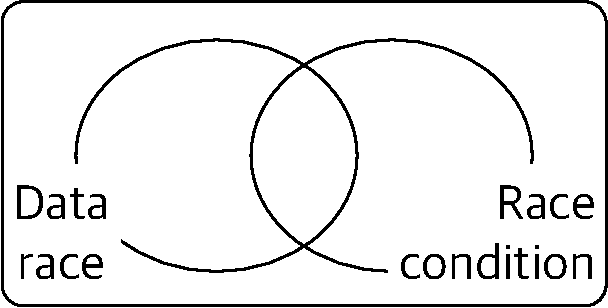
\includegraphics[width=0.45\linewidth]{fig/venndiagram.pdf}
%   \caption{Relation between data race and race condition. This paper
%     focuses on the striped region. \dr{I don't think we need this.}}
%   \label{fig:venndiagram}
% \end{figure}
%
Lastly, they are not a subset or a superset of one another. Although
there are race conditions that occur with data races, neither one is
the sufficient nor necessary condition for the other. Therefore, we
would argue that finding data races and finding race condditions are
complementary with each other.


\PP{Scope of this paper}
%
This paper focuses on finding race conditions instead of data races.

\dr{TODO: why? want to say finding race condition is more important,
  and existing approaches to find data races are limited}

\dr{TODO: need to say the importance of observing erroneous outcomes}




%%% Local Variables:
%%% mode: latex
%%% TeX-master: "p"
%%% End:
